%! Author = sriadityavedantam
%! Date = 4/8/26

\section{Local Divisors}

\begin{definition}[Cartier Divisor]
    A Cartier divisor is a locally principal Weil divisor.
\end{definition}

Let $X = \bigcup U_i$ be an affine open cover.
A divisor $D\in \Div(X)$ is called locally principal if $D|_{U_i}$ is principal for each $i$.
If $X = \pp^1$ and $D = (0)$, then $D$ is not principal globally, but it is locally principal.
Indeed, take the affine chart $\aa^1_t = \{t \neq \infty\}$.
Then $\pp^1 = \aa^1_t \cup \aa^1_u$ with $t = \frac{1}{u}$.
The divisor $D = \{t = 0\}$ is principal on $\aa^1_t$, and $D \cap \aa^1_u = \varnothing$.
Thus $D$ is locally principal.
The group of Cartier divisors is denoted $\Ca(X)$.
We define
\[
    \CaCl(X) \coloneqq \Ca(X)/\{\text{principal divisors}\}.
\]
This group is important since
\[
    \CaCl(X) \cong \mathrm{Pic}(X),
\]
the Picard group of $X$, which consists of line bundles up to isomorphism.

\begin{theorem*}{
    If $X$ is smooth, then every Weil divisor is Cartier.
}
\end{theorem*}

An example of a Weil divisor that is not Cartier is
\[
    X = \{xy = z^2\} \subseteq \c^3.
\]

\begin{figure}[H]
    \centering
    \captionsetup{justification=centering}

    \tikzset{every picture/.style={line width=0.75pt}}

    \begin{tikzpicture}[x=0.75pt,y=0.75pt,yscale=-1,xscale=1]
        \draw    (102,56) -- (206.41,222) ;
        \draw    (209,56) -- (109.07,218) ;
        \draw    (109.07,218) .. controls (122,239) and (166,244) .. (206.41,222) ;
        \draw  [dash pattern={on 4.5pt off 4.5pt}]  (109.07,218) .. controls (128,198) and (190,198) .. (206.41,222) ;
        \draw    (102,56) .. controls (120.93,36) and (192.59,32) .. (209,56) ;
        \draw    (102,56) .. controls (114.93,77) and (168.59,78) .. (209,56) ;

        \draw    (308,233) -- (548,233) ;
        \draw    (428,221) -- (428,245) ;
        \draw    (427,37) .. controls (450,93) and (449,111) .. (426,146) ;
        \draw    (427,101) .. controls (450,157) and (449,175) .. (426,210) ;
        \draw    (359,50) .. controls (399,20) and (344,189) .. (384,159) ;
        \draw    (326,50) .. controls (366,20) and (311,189) .. (351,159) ;
        \draw    (293,55) .. controls (333,25) and (278,194) .. (318,164) ;
        \draw    (457,51) .. controls (497,21) and (442,190) .. (482,160) ;
        \draw    (492,44) .. controls (532,14) and (477,183) .. (517,153) ;
        \draw    (524,48) .. controls (564,18) and (509,187) .. (549,157) ;

        \draw (556,222.4) node [anchor=north west][inner sep=0.75pt]    {$\aa^1_z$};
        \draw (424,246.4) node [anchor=north west][inner sep=0.75pt]    {$0$};
        \draw (400,14.4) node [anchor=north west][inner sep=0.75pt]    {$xy=0$};
        \draw (493,190) node [anchor=north west][inner sep=0.75pt]   {Singular point in $X$};
        \draw (570,106) node [anchor=north west][inner sep=0.75pt]   {Fibers};
    \end{tikzpicture}

    \caption{An affine surface with a singular point.}
\end{figure}

We have
\[
    f^{-1}(0) = \{xy = 0\} = \{x = 0\} \cup \{y = 0\}.
\]
Let $D = \{y = 0\} \subseteq f^{-1}(0)$.
We claim that $D$ is not Cartier.
Observe that
\[
    xy = z^2 \quad \Rightarrow \quad y = \frac{z^2}{x}.
\]
Thus along $D$, we have $\{y = 0\} = \{z = 0\}$.
The function $y$ vanishes to order $2$ along $D$, so
\[
    \nu_D(y) = 2.
\]
Hence
\[
    \div(y) = 2D.
\]
This shows $D$ is not principal, and in fact not Cartier.
When defining $\div(f) = \sum \nu_C(f)\,C$, we choose $U\subset X$ such that $C\cap U = \{\pi = 0\}$.

\begin{figure}[H]
    \centering

    \tikzset{every picture/.style={line width=0.75pt}}

    \begin{tikzpicture}[x=0.75pt,y=0.75pt,yscale=-1,xscale=1]
        \draw   (194,65) -- (503.75,65) -- (503.75,242) -- (194,242) -- cycle ;
        \draw   (253.88,99.21) -- (443.88,99.21) -- (443.88,207.79) -- (253.88,207.79) -- cycle ;
        \draw    (219,242) .. controls (515,199) and (168,130) .. (507,125) ;

        \draw (273,114.4) node [anchor=north west][inner sep=0.75pt]    {$\aa^2$};
        \draw (207,78.4) node [anchor=north west][inner sep=0.75pt]    {$\pp^2$};
    \end{tikzpicture}
\end{figure}

Take $\pi$ such that the ideal of functions vanishing on $D$ is generated by $\pi$.

\subsection{Q-Factorial}

\begin{definition}[Q-Factorial]
    A quasi-projective variety $X$ is Q-factorial if for every Weil divisor $D$, there exists $n\in \n$ such that $nD$ is Cartier.
\end{definition}

Recall in the example $X = \{xy = z^2\}$, we have $\div(y) = 2D$, which is Cartier.
If $X$ is an affine \textbf{\textit{toric variety}}, then $X$ is Q-factorial if and only if its fan is \textbf{\textit{simplicial}}.

\begin{figure}[H]
    \centering
    \captionsetup{justification=centering}

    \tikzset{every picture/.style={line width=0.75pt}}

    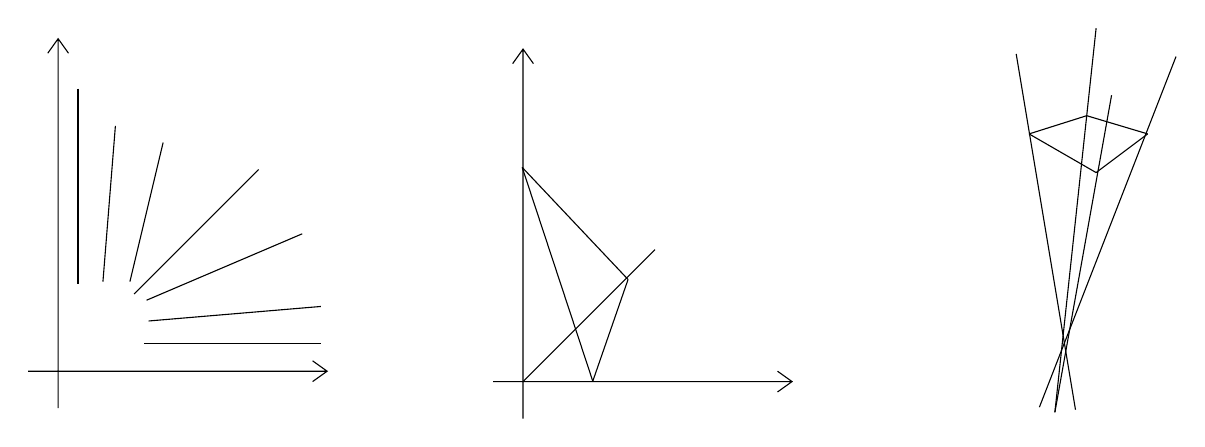
\begin{tikzpicture}[x=0.75pt,y=0.75pt,yscale=-1,xscale=1]
        \draw  (43,208.2) -- (187,208.2)(57.4,48) -- (57.4,226) (180,203.2) -- (187,208.2) -- (180,213.2) (52.4,55) -- (57.4,48) -- (62.4,55)  ;
        \draw    (67,72) -- (67,166) ;
        \draw    (184,195) -- (99,195) ;
        \draw    (184,177) -- (101,184) ;
        \draw    (154,111) -- (94,171) ;
        \draw    (85,90) -- (79,165) ;
        \draw    (175,142) -- (100,174) ;
        \draw    (108,98) -- (92,165) ;

        \draw  (267,213.2) -- (411,213.2)(281.4,53) -- (281.4,231) (404,208.2) -- (411,213.2) -- (404,218.2) (276.4,60) -- (281.4,53) -- (286.4,60)  ;
        \draw    (281.4,213.2) -- (345,149.6) ;
        \draw    (281,110) -- (315,213) ;
        \draw    (281,110) -- (332,164) ;
        \draw    (332,164) -- (315,213) ;

        \draw    (537.63,228) -- (557.5,42.95) ;
        \draw    (530.18,225.52) -- (596,56.61) ;
        \draw    (547.56,226.76) -- (519,55.37) ;
        \draw    (537.63,228) -- (564.95,75.24) ;
        \draw    (525.21,93.87) -- (552.97,85.09) ;
        \draw    (552.97,85.09) -- (582.34,93.87) ;
        \draw    (582.34,93.87) -- (557.5,112.5) ;
        \draw    (557.5,112.5) -- (525.21,93.87) ;
    \end{tikzpicture}

    \caption{From left to right: $\aa^2$, $\aa^3$, $\aa^4$: a conifold singularity which is not Q-factorial.}
\end{figure}